% ============================================================================
% IEEE paper source. Single source, one flag below switches the target format:
%   [conference]  -> IEEE conference (2 columns, ~8-12 pages)  [default]
%   [journal]     -> IEEE journal (TSE / IEEE Access)
% Build:  latexmk -pdf main.tex      (or: pdflatex; bibtex; pdflatex; pdflatex)
% ============================================================================
\documentclass[conference]{IEEEtran}
% \documentclass[journal]{IEEEtran}   % <- switch target here

\usepackage[T1]{fontenc}
\usepackage[utf8]{inputenc}
\usepackage{graphicx}
\usepackage{amsmath,amssymb}
\usepackage{booktabs}
\usepackage{array}
\usepackage{xcolor}
\usepackage[hidelinks]{hyperref}
\usepackage{url}

\newcommand{\pct}{\%}
\graphicspath{{figures/}}

\begin{document}

\title{Exact Reach Probabilities Explain and Predict\\
Generator Tradeoffs in Stateful Authorization Testing}

\author{\IEEEauthorblockN{Ignacio Peyrano}
\IEEEauthorblockA{Universidad Austral\\
Email: impeyrano@mail.austral.edu.ar}}

\maketitle

\begin{abstract}
Two kinds of test generators are used against stateful APIs: random generators and
generators that mutate valid workflows. Neither wins in general. Workflow mutation finds
defects that need several prior steps, and random programs find shallow scope violations
faster. We show that this tradeoff can be computed before any campaign runs. For an
authored appointment/payment service, we record the exact transition table of the real
HTTP/SQL backend over its 175-action campaign domain; from that table an exact dynamic
program gives each generator's probability of detecting a defect within a call budget.
The table is validated three ways: the unchanged campaign code reproduces all 2{,}740
recorded campaigns field for field; 8{,}750 transitions reached by real action paths
match the table; and a corrupted table fails 19 of 20 replays. With 1{,}000 seeds per
condition, valid workflow banks raise detection of capacity, payment and refund defects
from 0--13\% to 43--79\% at 120 calls, while cross-scope reading moves the other way
(99.5\% random vs.\ 30.2\% workflow mutation). In a prospective test, predictions derived
only from a specification model and frozen by hash reproduce every generator ordering on
14 systematically generated mutants. On OWASP crAPI, a service authored by others, frozen
specification-derived predictions reproduce all nine generator orderings against 450 live
campaigns with no cell deviating at $p<0.05$, and the generator fingerprint differs from
the authored service exactly as the model predicts. The contribution is a method that
turns generator choice from trial into computation; it is not a new fuzzing algorithm, a
security proof, or a claim of superiority over any tool.
\end{abstract}

\begin{IEEEkeywords}
software testing, REST API fuzzing, authorization, stateful testing, test generation,
reach probability, reproducibility
\end{IEEEkeywords}

\section{Introduction}
Authorization in business APIs depends on more than the operation name. It depends on
who calls, on which resource, and after which history. A refund can be legitimate once
and a violation the second time. A confirmation is legitimate only after payment. A read
is legitimate only within the caller's scope.

Test generators for stateful APIs differ in how they reach such histories: random
programs sample operations and arguments independently; workflow-seeded generators mutate
known valid tasks; and feedback-guided generators keep a corpus of programs indexed by
abstract observations \cite{r9,r10,r11,r12,r13,r19}.

Our earlier evaluations of these generators, over several fixtures and phases, gave a
consistent but unexplained pattern. Workflow mutation won on repeated refunds, unpaid
confirmation and overbooking. Random programs won on cross-scope reads. Richer feedback
helped some defects and hurt others. A list of per-property wins and losses does not tell
a practitioner what to run next, and with 10--30 seeds per condition many differences
were not statistically resolvable.

This paper replaces that list with a computation. For a finite campaign domain, the
probability that a generator detects a defect within a budget is determined by two
things: the service's transition structure and the generator's program distribution. Both
can be computed exactly. The \emph{minimal witness depth}, the number of calls in the
shortest violating history, is a useful proxy for the comparison between random programs
and workflow mutation. The quantity that decides the comparison, however, is the
generator's \emph{reach probability} for the violating histories.

\noindent\textbf{Contributions.}
\begin{enumerate}
\item \emph{An exact reach analysis for stateful authorization testing.} We record
transition tables from the real HTTP/SQL backend. Episode and budget distributions are
computed exactly for random, prefix-extension and mutation generators, validated by exact
replay of 2{,}740 recorded campaigns, path-based fidelity checks, and an exhaustive check
of the mutation enumeration.
\item \emph{Effect sizes at resolvable precision.} Running the unchanged campaign code on
the tables with 1{,}000 seeds per condition settles contrasts that 30-seed experiments
could not; among them, corpus guidance underperforms uniform workflow mutation on
history-dependent defects.
\item \emph{A prospective test across the specification/implementation boundary.}
Predictions derived only from the specification model order the generators correctly on
14 systematically generated mutants and identify three as undetectable within the bounded
domain; and on OWASP crAPI, an externally authored service.
\item \emph{A public artifact} with tables, frozen predictions, raw campaigns and replay
commands.
\end{enumerate}

We do not claim a new fuzzing algorithm, security verification of any production system,
or superiority over any tool.

Each result is labeled with one of three tiers: \emph{pipeline validation} (the tables
and model reproduce what was recorded), \emph{exploratory} (analysis of designs and
defects that informed this work), and \emph{prospective} (predictions frozen before
execution on new defects).

\section{Related Work}
\textbf{Stateful REST testing.} RESTler infers producer--consumer dependencies and uses
execution feedback \cite{r9}; its security checkers test namespace, hierarchy and
use-after-free style rules \cite{r11}. EvoMaster generates REST tests with evolutionary
search \cite{r24}. Sahin, Zhang and Arcuri \cite{r19}, extending \cite{r27}, are the
closest work to our setting: they add authentication and access-control oracles, some
multi-call (one user creates a resource and another probes it), run in a post-processing
phase over the tests the search produced, and evaluate one generator on many APIs
(including crAPI). They do not compare generators and do not model how likely a generator
is to reach a violation, and their oracles do not cover history-dependent business
violations such as repeated refunds, confirmation before payment or capacity --- which
are our focus. RESTTESTGEN \cite{r12}, mass-assignment testing \cite{r13},
specification-based access-control detection \cite{r18} and Schemathesis \cite{r25} add
nominal/error scenarios, vulnerability-specific oracles and schema-derived property
checks. Our generators and oracles have these antecedents; our contribution is to explain
and predict \emph{which} generator detects a given history-dependent defect.

\textbf{Probabilistic analyses of testing.} Arcuri, Iqbal and Briand give closed-form
results, framed as a coupon-collector problem, for the time random testing needs to reach
targets and for how predictable its reruns are \cite{r21}; our random-generation reach
probability is the same quantity made exact for one concrete stateful service rather than
a closed form over targets. B\"ohme and Paul model testing as sampling from abstract
error-based input partitions and derive bounds on the cost per test beyond which random
testing is more efficient than systematic partition testing on average \cite{r22}.
Probabilistic Concurrency Testing defines bug depth and gives detection bounds in terms
of depth \cite{r20}; our use of minimal witness depth follows that tradition. Sequence
covering arrays target $t$-way event orders \cite{r26}. Those analyses work with abstract
partitions, targets and parameters; ours computes exact per-generator detection
distributions over a transition table recorded from a concrete stateful implementation,
and contrasts random generation with workflow-seeded mutation and corpus guidance under a
shared budget.

\textbf{Evaluation practice.} We follow guidance on repeated randomized trials and on
separating detected inputs from distinct defects \cite{r17}. From \cite{r23} we adopt the
Vargha--Delaney $A_{12}$ effect size and its advice to report raw $p$-values; our paired
binary detection counts additionally use an exact McNemar test with Holm-adjusted
$p$-values (McNemar suits paired success/failure outcomes, which differ from the
continuous performance measures \cite{r23} centers on).

\textbf{Enabledness abstractions.} Enabledness-preserving abstractions \cite{r3,r4,r14}
support contract validation and coverage. Our earlier counterexample \cite{r1,r2} shows
that one particular global enabledness projection merges states that need different
authorization decisions; it does not refute those complete methods, and it now appears
only as background (Appendix~\ref{app:earlier}).

\section{Systems, Oracles and Threat Model}
\textbf{TurnoSalon} is the primary system, a FastAPI/SQLite service with two salon
branches, two customers and two staff members. Its business rules: reservations occupy
one unit of slot capacity; payments debit server-priced synthetic credit; confirmation
requires payment; cancellation releases capacity; and a staff refund credits the customer
exactly once. Identities are resolved from signed sessions, and writes commit in
independent SQLite transactions.

A separate specification oracle derives the expected status code, business state and
output for every call, then checks invariants over capacity, payment, refunds and ledger
balance. The oracle imports no implementation code.

The campaign domain is finite: 7 operations, 5 principals (including an anonymous one)
and 5 resource identifiers, giving 175 actions; programs of at most 8 actions; 120 calls
per campaign, with 480 as a sensitivity condition. The assumed attacker chooses
operations and identifiers with fixture credentials, including foreign identifiers and
repeated calls. Out of scope: resource creation, concurrency within campaigns, identity
management and server compromise; concurrent contracts are tested separately
(Appendix~\ref{app:earlier}).

\textbf{Reviewed defects.} Four deliberate mutants each omit one guard: booking read
scope, slot capacity, payment before confirmation, and the already-refunded check. They
were reviewed and used across phases v0.5--v0.8, informed this work, and are therefore
exploratory evidence.

\textbf{Systematic mutants (prospective).} We parse \texttt{SalonService.read} and
\texttt{SalonService.transition} and remove each top-level disjunct of every
\texttt{if\,...:\,raise} guard. This yields 18 sites with no hand selection; four coincide
with the reviewed defects, and the other 14 form the prospective set. Mutants are compiled
in memory and injected at adapter construction, and the measured source is never edited.

\textbf{Secondary fixtures.} A synthetic document-sharing service with eleven authored
defects (v0.2); an existing FastAPI/PostgreSQL backend by the same author, with a public
source subset and mitigation (v0.3--v0.4); and a scoped RESTler setup pilot (v0.7). They
are summarized in Appendix~\ref{app:earlier}.

\section{Generators and Campaigns}
All generators share one campaign loop. Before each program, the service is reset to the
fixture. Every executed call is charged against the budget. An episode stops at its first
oracle violation; the campaign stops at the first matching violation, or when the budget
is exhausted. The generators are: \textbf{random} (each program has a uniform length from
1 to 8, each action uniform over the 175-action domain); \textbf{valid replay} (one of
eight legitimate task programs, unchanged); \textbf{valid prefix + random}
(\texttt{seed\_extend}: a legitimate task followed by a uniform random suffix);
\textbf{mutation of valid bank} (\texttt{sequence\_uniform}: a uniform source and donor
task, then one of six generic operators --- field change, insert, duplicate, delete,
swap, splice); \textbf{mutation of random bank} (the same mutator on a length-matched
random bank); \textbf{corpus-guided mutation} (\texttt{sequence\_enabled},
\texttt{sequence\_enriched}: with probability 0.8 the source comes from a 64-entry FIFO
corpus keyed by coarse or enriched abstract transitions and scheduled toward rarely
selected keys, otherwise from the valid bank); and \textbf{balanced portfolio} (random
and valid-bank mutation, alternated by the calls each has consumed).

Every generator except random first executes its bank as a charged bootstrap (24 calls
for the valid bank). The corpus engines therefore differ from uniform mutation in source
selection, eviction and scheduling, not only in their feedback key.

\section{Exact Reach Analysis}
\subsection{Recorded transition tables}
For each service variant we run a breadth-first exploration. From each state, every one
of the 175 actions is executed through the real HTTP application and SQL database, and we
record the response, the next business snapshot and the oracle verdict. States are written
into a disposable database before each action. Only states reached through violation-free
transitions are expanded, because episodes stop at the first violation; levels 0--7 are
expanded, covering every program of up to eight actions. For the corrected service this
reaches 723 expandable states and 126{,}525 recorded transitions; exploration takes about
70 seconds per variant on 14 processes, and parallel and sequential exploration produce
identical tables.

\subsection{Episode and budget distributions}
Given a table and a target property, the following episode distributions are computed
exactly with rational arithmetic, as $P(\text{detect at call }c)$ and $P(\text{stop
without detection after }c\text{ calls})$: \emph{random episodes} by forward dynamic
programming over states, for each program length; \emph{mutation episodes} as the exact
output distribution of the mutation operator, enumerated over every source/donor pair (a
unit test drives the real mutator through every random-choice path and checks the
enumerated distribution is identical); and \emph{prefix extension} as the deterministic
prefix followed by a random suffix. A budget dynamic program combines i.i.d.\ episodes
with the deterministic charged bootstrap, giving the distribution of the first-failure
call index, from which we obtain $P(\text{detect within }B)$ and the expected capped
effort. This is exact for every generator except the corpus and portfolio engines, whose
episodes are not i.i.d.

\subsection{Validation (pipeline tier)}
\textbf{Exact replay.} We ran the unchanged v0.5, v0.6 and v0.8 campaign code on the
tables. All 2{,}740 recorded campaigns, across eight generators, five variants and two
budgets, matched their archives in all 19 recorded fields (complete traces, responses,
minimized witnesses and corpus statistics). As a negative control, a table with one
corrupted status code fails 19 of 20 replays. \textbf{Path fidelity.} For 10 sampled
states per variant we reset the service, executed the real action path leading to the
state (no restoration), and compared all 175 transitions against the table: 8{,}750 of
8{,}750 matched. \textbf{Consistency of predictions.} Across 48 recorded cells (study
$\times$ generator $\times$ defect $\times$ budget), observed detections are consistent
with the exact probabilities: the minimum two-sided binomial $p$ is 0.07, and 31 cells are
informative ($0.02<p<0.98$). This is expected and confirms the pipeline; it is not
independent predictive evidence.

\subsection{Shortest witnesses and reach}
For each variant, breadth-first search over clean transitions gives the shortest violating
history and the number of distinct shortest witnesses; this depth does not depend on any
campaign and, for the four reviewed defects, equals the length of every deletion-minimized
witness recorded in v0.5--v0.8 (Table~\ref{tab:depth}).

\begin{table}[t]
\caption{Shortest witnesses for the reviewed defects.}
\label{tab:depth}
\centering
\footnotesize
\begin{tabular}{@{}lcc@{}}
\toprule
Defect & Depth & Distinct shortest witnesses \\
\midrule
Cross-scope read & 1 & 8 \\
Overbooking & 2 & 16 \\
Unpaid confirmation & 2 & 8 \\
Repeated refund & 5 & 16 \\
Corrected service & --- & 0 \\
\bottomrule
\end{tabular}
\end{table}

Depth explains why random generation fails on deep defects: a uniform random program
contains a specific five-action history with probability on the order of $175^{-5}$. Depth
does not, by itself, rank generators that share structure with the witness; the relevant
quantity is each generator's per-episode reach probability.

\section{Experimental Design}
Table~\ref{tab:design} summarizes the data and purpose of each tier. The surrogate runs
use the original campaign implementations; the table adapter falls back to the real
backend for any state outside the table, and no fallback occurred (0 misses).

\begin{table}[t]
\caption{Experimental tiers.}
\label{tab:design}
\centering
\footnotesize
\begin{tabular}{@{}p{1.1cm}p{3.3cm}p{2.6cm}@{}}
\toprule
Tier & Data & Purpose \\
\midrule
Pipeline & 2{,}740 recorded campaigns (v0.5/6/8); 8{,}750 path checks & Tables and model reproduce recordings \\
Exploratory & Campaign code on tables, 1{,}000 fresh seeds/cell & Effect sizes for all generators \\
Exploratory & Planned v0.6/v0.8 contrasts, 30 seeds (McNemar, $A_{12}$, Holm) & Record of planned tests \\
Exploratory & Document benchmark, Monte Carlo, 10{,}000 episodes/cell & Second fixture for reach \\
Prospective & 14 systematic mutants, frozen predictions, 1{,}260 campaigns & Order and calibration on new defects \\
\bottomrule
\end{tabular}
\end{table}

\section{Results}
\subsection{Initial knowledge and perturbation (exploratory)}
Table~\ref{tab:detect} reports detection within 120 calls, 1{,}000 seeds per cell. With
the mutator held fixed, a valid bank in place of a length-matched random bank raises
detection of the three history-dependent defects by 43--76 points and lowers cross-scope
reading by 45 points. Reach explains both directions: valid tasks place the payment,
cancellation and refund prefixes one mutation from the witness, but never pair a principal
with a foreign booking, so a scope witness needs a field mutation the random generator
gets for free on every call. Appending random suffixes to valid prefixes recovers most of
the scope detection but little of the history detection; replay without perturbation
detects nothing.

\begin{table*}[t]
\caption{Detection within 120 calls, 1{,}000 seeds per cell.}
\label{tab:detect}
\centering
\footnotesize
\begin{tabular}{@{}lcccc@{}}
\toprule
Generator & Cross-scope read & Overbooking & Unpaid confirmation & Repeated refund \\
\midrule
Random & 99.5\% & 13.1\% & 6.2\% & 0.0\% \\
Random after charged warmup & 98.8\% & 11.7\% & 4.7\% & 0.0\% \\
Valid replay & 0.0\% & 0.0\% & 0.0\% & 0.0\% \\
Valid prefix + random & 88.2\% & 14.2\% & 7.3\% & 5.8\% \\
Mutation of random bank & 75.2\% & 3.2\% & 1.5\% & 0.0\% \\
Mutation of valid bank & 30.2\% & 78.7\% & 73.0\% & 42.9\% \\
Corpus-guided, coarse key & 29.1\% & 45.8\% & 49.3\% & 22.0\% \\
Corpus-guided, enriched key & 28.1\% & 66.5\% & 47.3\% & 23.5\% \\
\bottomrule
\end{tabular}
\end{table*}

The planned 30-seed contrasts point the same way. After Holm adjustment within each
study's family (24 in v0.6, 16 in v0.8), all valid-versus-random-bank contrasts remain
significant (exact McNemar, Holm $p\le0.025$); $A_{12}$ on capped calls ranges from 0.15
to 0.84.

\subsection{Corpus guidance and feedback keys (exploratory)}
Table~\ref{tab:corpus} gives paired differences from uniform valid-bank mutation, in
percentage points with 95\% intervals over the same 1{,}000 seeds. In this configuration
corpus guidance never improves on uniform mutation of the valid bank, and on repeated
refunds the deficit grows with the budget. The contrast changes source-selection
probability, FIFO eviction and rare-key scheduling together, so it does not isolate the
value of feedback in general. Holding everything else fixed, the enriched key beats the
coarse key only on overbooking ($+20.7\pm3.6$ points at 120 calls); on the other three
defects the 95\% intervals include zero. With 30 seeds the overbooking contrast had raw
$p=0.0063$ and Holm-adjusted $p=0.063$ --- a matter of power, not evidence of no effect.

\begin{table*}[t]
\caption{Corpus engines minus uniform valid-bank mutation (percentage points, 95\% interval).}
\label{tab:corpus}
\centering
\footnotesize
\begin{tabular}{@{}llcccc@{}}
\toprule
Budget & Engine & Read & Overbooking & Unpaid confirmation & Refund \\
\midrule
120 & Coarse corpus   & $-1.1\pm3.8$ & $-32.9\pm3.9$ & $-23.7\pm4.1$ & $-20.9\pm3.9$ \\
120 & Enriched corpus & $-2.1\pm3.8$ & $-12.2\pm3.8$ & $-25.7\pm4.0$ & $-19.4\pm3.9$ \\
480 & Coarse corpus   & $-5.3\pm3.4$ & $-4.7\pm1.3$  & $-5.2\pm1.4$  & $-33.6\pm3.4$ \\
480 & Enriched corpus & $-7.2\pm3.5$ & $-1.8\pm0.8$  & $-6.5\pm1.6$  & $-32.7\pm3.5$ \\
\bottomrule
\end{tabular}
\end{table*}

\textbf{Bank sensitivity.} The valid-bank advantage is not a property of ``valid tasks''
in the abstract; it is a property of whether the bank contains a task whose prefix reaches
the witness. Recomputing the exact 120-call order with one task template removed makes
this precise (Table~\ref{tab:bank}). The depth-1 scope read is bank-independent; for each
history defect, removing the single template that supplies the witness prefix collapses
mutation's detection and flips the winner. The reach model predicts this: mutation only
wins when a bank task sits one operator from the witness. This exposes the dependence on a
hand-chosen bank and shows the model explains it rather than assuming it.

\begin{table}[t]
\caption{Bank sensitivity: effect of removing the enabling template.}
\label{tab:bank}
\centering
\footnotesize
\begin{tabular}{@{}lp{1.3cm}p{3.1cm}@{}}
\toprule
Defect & Full bank & After removing the enabling template \\
\midrule
Cross-scope read & random wins & stable under every removal \\
Overbooking & mutation 0.80 & drop rebook task $\rightarrow$ 0.03; prefix extension wins \\
Unpaid confirmation & mutation 0.71 & drop confirm task $\rightarrow$ 0.01; prefix extension wins \\
Repeated refund & mutation 0.42 & drop refund task $\rightarrow$ 0.00 \\
\bottomrule
\end{tabular}
\end{table}

\subsection{Budget and portfolio (exploratory)}
At 120 calls the balanced portfolio lies between its components on every defect
(Table~\ref{tab:portfolio}); at 480 calls it reaches 94--100\% on the first three defects
and 72.2\% on refund, against 92.5\% for mutation alone. The exact model gives the whole
detection curve, not only two budgets (Fig.~\ref{fig:curves}). The observed 1{,}000-seed
fractions fall on the predicted curves, and for these defects the generator ranking does
not change with the budget: random dominates the depth-1 scope read at every budget, and
valid-bank mutation dominates the history-dependent defects at every budget. A
practitioner choosing a generator need not guess the budget at which the ranking flips,
because here it does not flip after the first few calls. These values also explain an
apparent inconsistency between phases: valid-bank mutation detected cross-scope reads in
8/30 campaigns in v0.6 and 14/30 in v0.8 under identical settings, and the exact
probability is 0.30, so the v0.8 result was a favorable draw.

\begin{table}[t]
\caption{Detection at 120 calls: portfolio vs.\ components.}
\label{tab:portfolio}
\centering
\footnotesize
\begin{tabular}{@{}lccc@{}}
\toprule
Defect & Portfolio & Random & Valid-bank mutation \\
\midrule
Cross-scope read & 93.7\% & 99.5\% & 30.2\% \\
Overbooking & 48.6\% & 13.1\% & 78.7\% \\
Unpaid confirmation & 39.9\% & 6.2\% & 73.0\% \\
Repeated refund & 16.7\% & 0.0\% & 42.9\% \\
\bottomrule
\end{tabular}
\end{table}

\begin{figure*}[t]
\centering
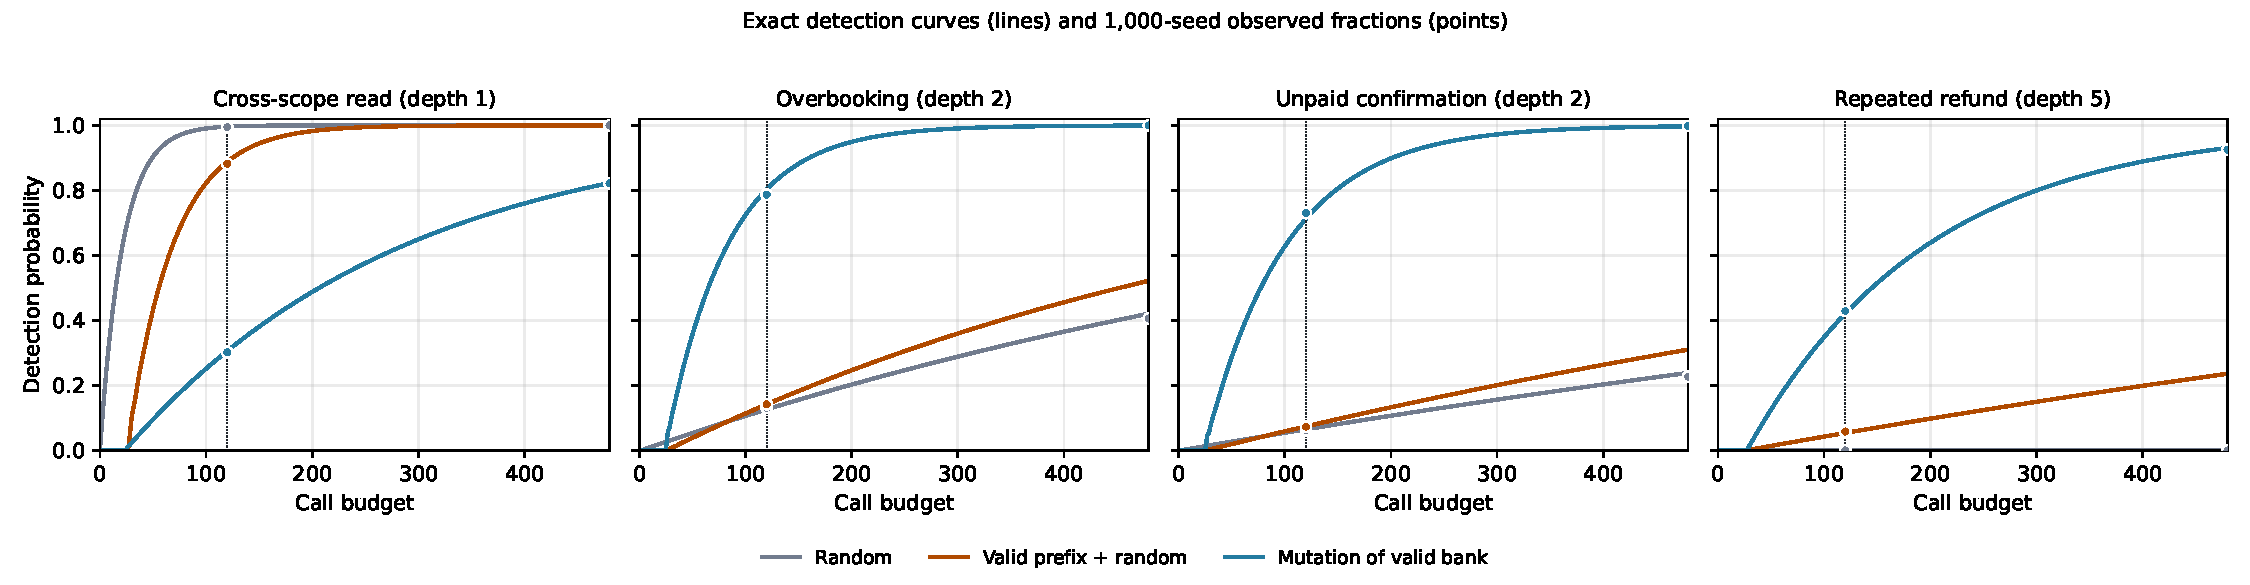
\includegraphics[width=\textwidth]{reach-curves.pdf}
\caption{Exact detection probability versus call budget (lines) with 1{,}000-seed observed
fractions (points) for the three main generators on the four reviewed defects. The dotted
line marks the 120-call budget.}
\label{fig:curves}
\end{figure*}

\subsection{Second fixture: the document benchmark (exploratory)}
The document service has a larger action domain (recipients and approval tokens), and its
legacy random generator differs from the business generator. We estimated per-episode
detection probabilities with the unchanged components, over 10{,}000 episodes per defect
and generator. Minimal witness depth separates the extremes: sharing overwrite (depth 3)
and approval replay (depth 5) are found by valid-bank mutation in 10/10 runs, while random
finds them in at most 1/10 (per-episode reach $\le0.0001$ vs.\ $\approx0.026$ for
mutation); unauthorized update (depth 1) has reach 0.348 for random against 0.003 for
mutation (observed 10/10 vs.\ 6/10). Depth fails for wrong-recipient acceptance: it has
depth 2, yet random detected it in 8/10 runs and valid-bank mutation in 4/10, and the
per-episode reach ordering agrees with the observed direction (0.0083 vs.\ 0.0017). The
recorded minimal witnesses are an initiated share followed by acceptance from a principal
other than the pending recipient; from the valid bank either form needs one specific field
change in one of the two sharing tasks. The budget-level predicted gap is small (7.1 vs.\
6.3 expected detections out of 10) and $n=10$ cannot confirm the direction: this is post
hoc evidence that depth is only a proxy, not proof that reach is superior.

\subsection{Prospective test on systematic mutants}
The 14 prospective predictions were derived only from the specification model: for each,
the corresponding disjunct was removed from the oracle's expected-behavior function,
restricted to the operations the implementation guard covers. Before freezing, the
specification model was checked on the corrected service and the four reviewed defects; in
all five cases its state graph and violation sets were identical to the recorded
implementation tables. The predictions were committed by hash before any campaign ran. A
first execution exposed a harness defect (the compiled mutant had its own copy of the
exception class, turning every rejection into an HTTP 500); that run is preserved and
documented, the fix changed neither predictions nor analysis plan, and the injection is
now checked against the four known tables before any run.

Results of the second execution (Fig.~\ref{fig:calib}): \textbf{Generator order} --- all
26 pairs whose frozen probabilities differ by at least 0.1 were ordered correctly by the
observed counts. A depth-only rule (depth~1 $\rightarrow$ random beats workflow
generators; depth~$\ge2$ $\rightarrow$ workflow generators beat random) also gets the 15
random-versus-workflow pairs it can order, but the remaining 11 pairs compare prefix
extension with valid-bank mutation --- depth cannot order them, and the exact model orders
all 11 correctly. \textbf{Bounded-equivalent mutants} --- three mutants have no violating
program within eight actions; for each, the implementation table is identical to the
specification table and neither contains a violation, and they produced 0 detections in
270 campaigns. \textbf{Calibration} --- the frozen metric is the number of cells with
$p<0.05$ over all cells: 4 of 42 (about 2 expected by chance, so within sampling
variation). Restricting to the 20 cells with a non-degenerate prediction, a declared
secondary view, leaves 3. The four deviating sites were diagnosed, not assumed to be
noise: their implementation and specification graphs are identical, all recorded campaigns
replay exactly on the implementation tables, and re-running each deviating cell with
3{,}000--12{,}000 fresh seeds matches the frozen probabilities. We found no model error;
every deviation is a low-probability draw at $n=30$.

\begin{figure*}[t]
\centering
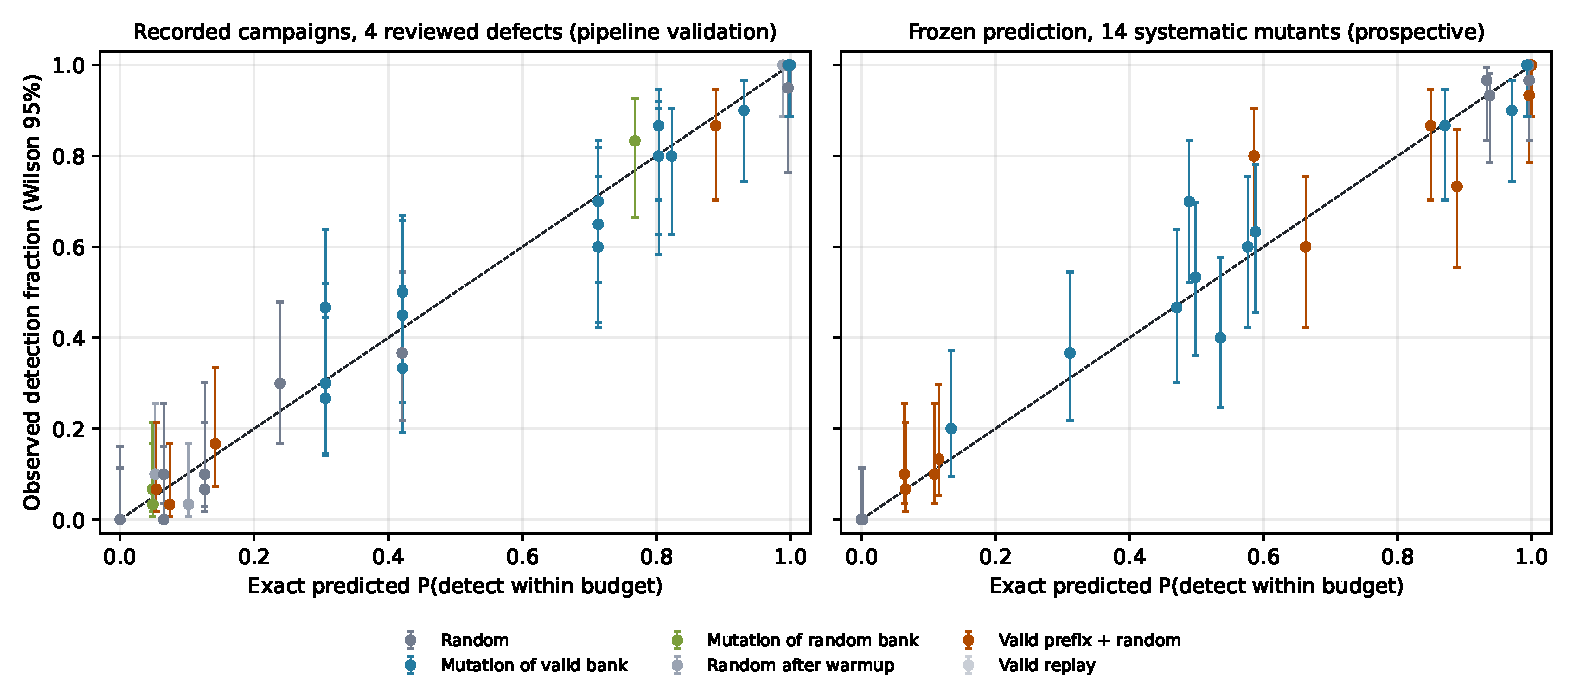
\includegraphics[width=\textwidth]{reach-calibration.pdf}
\caption{Exact predicted detection probability versus observed fraction with Wilson 95\%
intervals. Left: recorded campaigns on the four reviewed defects (pipeline validation).
Right: frozen specification-derived predictions for 14 systematic mutants (prospective).}
\label{fig:calib}
\end{figure*}

\subsection{Bounded exhaustive check of the corrected service}
For the corrected service, the table covers every program of up to eight actions over the
175-action domain, and no transition from any reachable clean state produces an oracle
violation, so no such program violates the oracle. The scope is exact with respect to the
recorded table --- this fixture, no resource creation, at most eight actions, and only
oracle-observable properties --- and the table equals the backend under the assumption
that behavior depends only on the observable snapshot (Section~\ref{sec:threats}), checked
on a 50-state path-fidelity sample.

\subsection{Earlier phases}
The earlier phases remain consistent with the reach account (Appendix~\ref{app:earlier}).
In the AoristoTech HTTP/PostgreSQL case, valid-task mutation detected repeated
cancellation (depth 2) in 10/10 runs against 0/10 for random, while random detected
foreign-store reads (depth 1) in 9/10 against 3/10. The RESTler setup pilot could not
reach the legitimate refund workflow within its budget, consistent with (though not
computed as) the near-zero reach of generators that cannot assemble the payment and
cancellation prefix.

\subsection{Independent service: OWASP crAPI (prospective)}
The strongest test of the method is a service this project did not author. OWASP crAPI is
an intentionally vulnerable application; we study its shop (orders, returns, refunds) at
pinned revision \texttt{700f03d1}, with every container pinned by digest. We write a
specification of its intended behavior from the documented challenges and the OpenAPI
descriptions (disclosing that the vulnerable view code was read first), and define a
finite domain of two customers and seven shop operations. Because crAPI contains several
real defects at once, we target five rule families and stop each episode only at its
target property. The exact reach model is computed per target from the specification, and
predictions were frozen by hash before any live campaign ran. We then ran 450 live
HTTP/SQL campaigns (3 generators $\times$ 5 targets $\times$ 30 seeds, budget 60) against
the unmodified crAPI shop, with the business oracle judging every transition. The only
environment change is pointing crAPI's unused external payment gateway at a dead port so
order reads do not stall; it never affects the oracle.

The frozen predictions reproduce all nine generator orderings whose probabilities differ
by at least 0.1, with no cell deviating from its predicted detection at $p<0.05$, and two
rule families with no reachable violation yield 0 of 30 for every generator, as predicted.
The generator fingerprint differs from the authored salon service, and the model predicted
the difference: crAPI's defects are shallow (reading another user's order is depth 1;
tampering with status or quantity is depth 2), so random and valid-prefix extension beat
valid-bank mutation on all three detected families --- the reverse of the salon
history-dependent defects. Order-privacy (depth 1) is won by random (28/30); order
tampering and refund-without-return (depth 2) by valid-prefix extension (24/30 and 17/30);
valid-bank mutation is weakest on each (9, 8 and 3 of 30), because crAPI's valid tasks do
not sit one mutation from these witnesses. This is prediction across the
specification/implementation boundary on a service of another author; crAPI remains an
intentionally vulnerable training application with public challenges, so this is
implementation independence, not discovery of unknown defects.

\section{Discussion}
\textbf{A precomputation before fuzzing.} When the action domain is finite and the
specification is executable, a generator's detection probability for a hypothesized defect
can be computed before running it --- about one minute per mutant here. The practical use
is allocation: reach probabilities tell where random programs suffice (shallow scope
checks), where workflow seeds are necessary (payment and refund histories), and where
neither will succeed within a budget. Systematic guard-removal mutants of the
specification can stand in for unknown defects.

\textbf{Seeds are knowledge, and their placement matters.} The same valid tasks help when
mutated internally and barely help as a prefix to random suffixes. Mutation keeps the
dependency structure of the task while changing the critical step; a random suffix rarely
produces the specific repeated or out-of-order call.

\textbf{Corpus guidance needs evidence.} In this domain a coverage-style corpus diverts
effort away from the complete valid tasks whose single mutations reach the violations;
because the gap persists at four times the budget (large on refunds, smaller elsewhere) it
is not only a warmup cost. Other domains may favor corpus guidance. The broader point is
that a 30-seed experiment cannot resolve such differences, and an exact replica can.

\textbf{Why exact rather than bounded.} Analytic bounds such as PCT's \cite{r20} guarantee
a minimum detection probability as a function of depth. Our domain is small enough to
compute exact values, and exactness is what makes generators with the same depth
comparable. The cost is scale: the approach needs a finite action domain, resettable state
and tractable reachable state counts (723 here); abstraction or sampling would be required
beyond that.

\section{Threats to Validity}
\label{sec:threats}
\textbf{Construct.} Detection is measured against our specification oracle, and the
specification and implementation share an author; their identical state graphs on the
known variants show agreement, not independent correctness. The prospective predictions
come from the specification model, and the specification mutants are mapped to
implementation mutants by a hand-written table written with both in view. Graph identity
was verified for 12 variants (5 pre-freeze checks and the 7 diagnosed mutants), not for
the other 7 prospective mutants; where the graphs coincide, the prospective test measures
the fidelity of that mapping as much as a prediction crossing the
specification/implementation boundary. An independently authored service, where no such
mapping is possible, is the real test; crAPI is a step toward it. Reach probabilities are
defined for the campaign domain; arguments outside it (new resources, free-form payloads)
are not modeled.

\textbf{Internal.} The tables assume behavior depends only on the observable business
snapshot, because a state is reached by restoring that snapshot with SQL. Path-based
fidelity checks support this on 50 sampled states, not exhaustively. The assumption holds
here because booking identifiers are fixed, no resources are created, and execution is
single-threaded; it would break under concurrency, state kept outside the database,
timestamps, or identifiers whose value changes behavior. In crAPI the risk is higher:
sequences are not reset between the service's own calls and authentication carries state,
so the symbolic order binding is sound only while behavior does not depend on the concrete
order id, which is checked and stated there. The four reviewed defects shaped the method;
only the 14 systematic mutants are prospective. The valid-task bank is eight hand-written
programs; because the reserve/pay/cancel/refund template is exactly the repeated-refund
witness prefix, mutation is one insertion from that witness, and the bank-sensitivity
analysis recomputes the order with templates removed or added.

\textbf{External.} The authored systems are small and the mutant operator family
(guard-disjunct removal) is narrow, so real defects may be distributed differently. The
independent evaluation on OWASP crAPI removes the shared-authorship objection for the
implementation, but crAPI is still an intentionally vulnerable training application whose
defects are public, not an unseen-defect holdout, and its specification was written by us.

\textbf{Conclusion.} Surrogate effect sizes use 1{,}000 seeds per cell within one service
and describe search-seed variation, not variation across systems. The 30-seed planned
tests are reported with Holm adjustment as the original record, not the basis for the
effect sizes above.

\subsection{Future work}
Two external-tool comparisons are left as future work. First, a stronger RESTler
configuration, with a dictionary and authentication tuned until it reaches the legitimate
payment-and-cancellation workflow, so its detection can be compared under a matched budget
rather than the setup pilot. Second, a comparison with EvoMaster and its access-policy
oracles \cite{r19,r27} on the salon and crAPI services, the closest antecedent to our
setting. Both are infrastructure-heavy and neither would license a claim of general
superiority: the contribution here is predicting which generator detects which defect, not
outperforming a particular tool. A held-out service with unknown defects, and extension
beyond finite action domains via sampled rather than exact reach, are the other open
directions.

\section{Conclusion}
Generator tradeoffs in stateful authorization testing need not be found by trial. For a
finite domain, a generator's probability of exposing a history-dependent violation is
computable from the transition structure and the generator's program distribution. Minimal
witness depth is a useful proxy for that probability; the probability itself explains the
cases where depth fails, and, computed from a specification alone, it predicted the
generator order for new systematic defects and for an externally authored service before
execution. The same replica turns underpowered comparisons into precise ones: corpus
guidance in this service trails plain mutation of valid workflows. The method turns
generator choice from a lottery into a computation.

\section*{Artifact Availability}
Source, tables, raw campaigns, frozen predictions and figures are at
\url{https://github.com/PeyranoDev/semantic-gateway-lab}. The repository documents the
reproduction commands and maps claims to evidence. Full texts of \cite{r19,r21,r22,r23,r27}
were read; for \cite{r20,r24,r25,r26} only bibliographic metadata and abstracts were
verified.

\appendices
\section{Earlier Phases}
\label{app:earlier}
Table~\ref{tab:phases} lists the earlier phases and their role here. The enabledness
counterexample: let $\alpha_E$ map a state to the set of tool names enabled by existential
lifecycle conditions; if two states have equal $\alpha_E$ but different authorization
decisions for the same fully specified invocation, then no function of $(\alpha_E(s),a)$
reproduces the decision. Executable witnesses exist in the document service (one sharing
prefix designates Bob, the other Mallory) and in the salon service (confirmation of the
same booking). The feedback keys are used for search only, while the runtime and oracle
inspect full state.

\begin{table}[t]
\caption{Earlier phases.}
\label{tab:phases}
\centering
\footnotesize
\begin{tabular}{@{}lp{1.0cm}p{3.0cm}@{}}
\toprule
Phase & Campaigns & Role here \\
\midrule
v0.1--v0.2 & 1{,}080 & Document service; second fixture for reach; enabledness counterexample \\
v0.3--v0.4 & 120+ & AoristoTech; depth pattern in an existing backend \\
v0.5 & 640 & TurnoSalon; recorded campaigns replayed exactly \\
v0.6 & 1{,}200 & Component study; planned contrasts \\
v0.7 & 60 & RESTler setup pilot; no refund reachability \\
v0.8 & 900 & Fixed portfolio, budgets 120/480 \\
\bottomrule
\end{tabular}
\end{table}

\bibliographystyle{IEEEtran}
\bibliography{references}

\end{document}
